\begin{surferPage}[Cubica-Cayley]{Cubica lui Cayley}
    Aceast\u{a} suprafa\c{t}\u{a} cubic\u{a} (suprafa\c{t}\u{a} de grad $3$) apare de asemenea 
    \^{i}n galeria suprafe\c{t}elor simple. Are patru singularit\u{a}\c{t}i \^{i}n total, de tip con dublu. Este
    denumit\u{a} \^{i}n cinstea lui Arthur Cayley, care a studiat \^{i}n profunzime cubicele, in secolul XIX.
    
    Cu toate acestea, Ludwig Schl\"{a}fli este cel care \^{i}n 1863 a clasificat in mod sistematic aceste 
     suprafe\c{t}e, in functie de singularit\u{a}\c{t}ile lor. De exemplu, putem afla din articolul lui c\u{a} o
     suprafa\c{t}\u{a} cubic\u{a} nu poate avea mai mult de $4$ puncte singulare. A\c{s}adar: $\mu(3)=4$. 
    
    \^{I}n jurul anului 1900, Felix Klein a studiat formele posibile ale suprafe\c{t}elor cubice reale.
    Ideea lui era s\u{a} r\u{a}spund\u{a} la aceast\u{a} \^{i}ntrebare pentru cubica Cayley mai \^{i}nt\^{a}i, prin
    intermediul deform\u{a}rilor mici. Prin extinderea singularit\u{a}\c{t}ilor conului dublu,  a deconect\u{a}rii 
    sau a fuzion\u{a}rii de p\u{a}r\c{t}i, el a reu\c{s}it sa gaseasc\u{a} toate formele posibile. Iat\u{a} c\^{a}teva
    dintre ele:
    \vspace{0.3cm}
     \begin{center}
      \vspace{-0.2cm}
      \begin{tabular}{@{}c@{\ }c@{\ }c@{\ }c@{}}
        \begin{tabular}{@{}c@{}}
          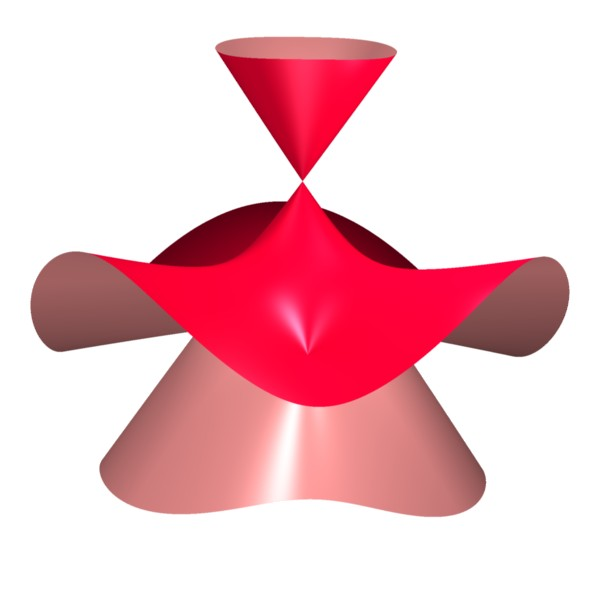
\includegraphics[width=1.35cm]{cayley_cubic_0}
        \end{tabular}
        &
        \begin{tabular}{@{}c@{}}
          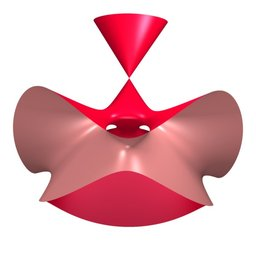
\includegraphics[width=1.35cm]{cayley_cubic_1}
        \end{tabular}
        &
        \begin{tabular}{@{}c@{}}
          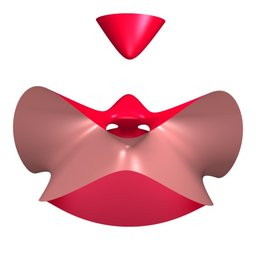
\includegraphics[width=1.35cm]{cayley_cubic_2}
        \end{tabular}
        &
        \begin{tabular}{@{}c@{}}
          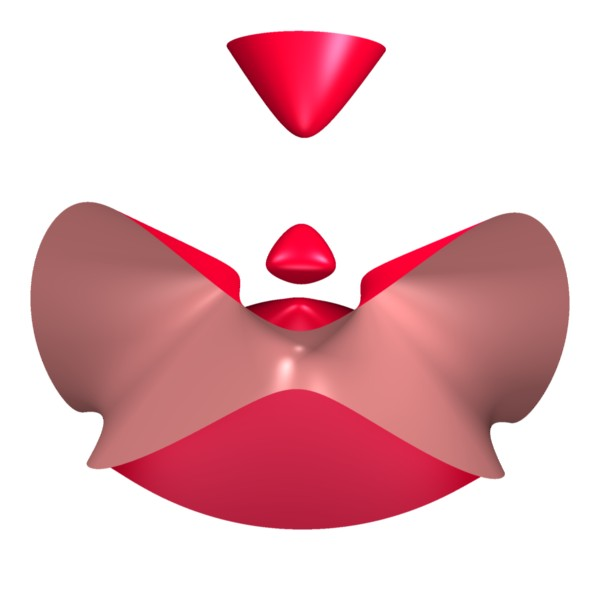
\includegraphics[width=1.35cm]{cayley_cubic_3}
        \end{tabular}
      \end{tabular}
    \end{center}
\end{surferPage}
